\documentclass[preview]{standalone}
\usepackage{caption}
\usepackage{tikz}
\usetikzlibrary{fit, arrows}
\captionsetup[figure]{labelformat=empty}

\begin{document}
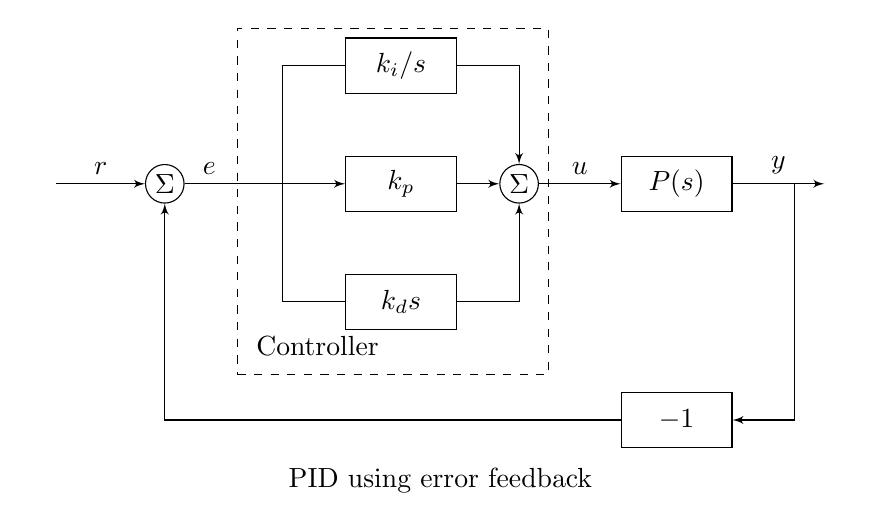
\begin{tikzpicture}[auto, node distance=1.5cm,>=latex']
  \tikzstyle{block} = [draw, rectangle, minimum height=2em, minimum width=4em]
  \tikzstyle{sum} = [draw, fill=white, circle, inner sep=0.5mm]
  \tikzstyle{tmp} = [coordinate]
  \node (input) {};
  \node [sum, right of=input] (sum) {$\Sigma$};
  \node [tmp, right of=sum] (ctrlleft) {};
  \node [block, right of=ctrlleft] (ctrlmid) {$k_p$};
  \node [block, above of=ctrlmid] (ki) {$k_i/s$};
  \node [block, below of=ctrlmid] (kd) {$k_ds$};
  \node [below left of=kd, yshift=0.5cm] (label) {Controller};
  \node [sum, right of=ctrlmid] (ctrlright) {$\Sigma$};
  \node [block, right of=ctrlright, xshift=0.5cm] (process) {$P(s)$};
  \node [tmp, right of=process] (split) {};
  \node [block, below of=process, yshift=-1.5cm] (minus1) {$-1$};
  \node [left=1cm, right of=split] (output) {};
  \node [fit=(input) (sum) (process) (minus1) (output), label=below:{PID using error feedback}] {};
  \node [draw, dashed, fit=(ctrlmid) (ki) (kd) (ctrlright) (label)] {};

  \draw [->] (input) -- node {$r$} (sum);
  \draw [->] (sum) -- node[above left, xshift=-0.5cm] {$e$} (ctrlmid);
  \draw (kd) -| (ctrlleft) |- (ki);
  \draw [->] (ki) -| (ctrlright);
  \draw [->] (kd) -| (ctrlright);
  \draw [->] (ctrlmid) -- (ctrlright);
  \draw [->] (ctrlright) -- node {$u$} (process);
  \draw [->] (process) -- node {$y$} (output);
  \draw [->] (split) |- (minus1);
  \draw [->] (minus1) -| (sum);
\end{tikzpicture}
\end{document}
